\documentclass[a4paper]{scrreprt}

% Uncomment to optimize for double-sided printing.
% \KOMAoptions{twoside}

% Set binding correction manually, if known.
% \KOMAoptions{BCOR=2cm}

% Localization options
\usepackage[english]{babel}
\usepackage[T1]{fontenc}
\usepackage[utf8]{inputenc}

% Quotations
\usepackage{dirtytalk}

% Enhanced verbatim sections. We're mainly interested in
% \verbatiminput though.
\usepackage{verbatim}

% PDF-compatible landscape mode.
% Makes PDF viewers show the page rotated by 90°.
\usepackage{pdflscape}

% Advanced tables
\usepackage{tabu}
\usepackage{longtable}

% Fancy tablerules
\usepackage{booktabs}

% Graphics
\usepackage{graphicx}

% Current time
\usepackage[useregional=numeric]{datetime2}

% Float barriers.
% Automatically add a FloatBarrier to each \section
\usepackage[section]{placeins}

% Importing CSV into tables
\usepackage{csvsimple}

% Custom header and footer
\usepackage{fancyhdr}

\usepackage{geometry}
\usepackage{layout}

% Math tools
\usepackage{mathtools}
% Math symbols
\usepackage{amsmath,amsfonts,amssymb}
\usepackage{amsthm}

\DeclarePairedDelimiter\abs{\lvert}{\rvert}

\pagestyle{plain}
% \fancyhf{}
% \lhead{}
% \lfoot{}
% \rfoot{}
% 
% Source code & highlighting
\usepackage{listings}

% SI units
\usepackage[binary-units=true]{siunitx}
\DeclareSIUnit\Molar{\textsc{m}}
\DeclareSIUnit\mole{mol}
\DeclareSIUnit\rpm{rpm}
\DeclareSIUnit\cfu{cfu}

\usepackage{mhchem}

\newcommand{\mysubject}{2115 - Lab course biochemistry 2}
\newcommand{\mytitle}{Expression, purification and characterization of superoxide oxidase SOO}

% Convenience commands
\newcommand{\mailsubject}{\mysubject{} \mytitle{}}
\newcommand{\maillink}[1]{\href{mailto:#1?subject=\mailsubject}
                               {#1}}

% Should use this command wherever the print date is mentioned.
\newcommand{\printdate}{\today}

\subject{\mysubject{}}
\title{\mytitle{}}

\author{Michael Senn \maillink{michael.senn@students.unibe.ch} - 16-126-880}

\date{\printdate}

% Needs to be the last command in the preamble, for one reason or
% another. 
\usepackage{hyperref}


\begin{document}
\maketitle

\chapter{Procedure\cite{skript_ballmoos}}

The listed steps are based on the provided script, with changes where we
deviated from what was written.

\section{Expression}

Expression was done by the assistants ahead of time, the corresponding steps of
the protocol are only listed for completeness' sake.

\begin{itemize}
	\item From a freshly transformed plate (plasmid: pET28) of the given
		membrane protein target in BL21 pLysS strain, inoculate
		\SI{30}{\ml} LB medium containing \SI{30}{\ug \per \ml}
		kanamycin (kan) for the expression of different proteins. Leave
		shaking overnight (ON) at \SI{37}{\celsius}. This pre-culture
		volume is suitable for \SI{1.5}{\l} culture grow-up.

	\item Prepare and autoclave \SI{1.5}{\l} of LB medium overnight so that
		the medium remains warm on the next day.

	\item To each \SI{1.5}{\l} bottle, add \SI{30}{\ml} of pre-culture
		inoculum, the appropriate antibiotics and incubate in a water
		bath with a controlled temperature at \SI{37}{\celsius}. We
		used a new device called LEX48 for bacteria growing in which
		shaking is replaced by air bubbling directly in the medium.

	\item Check the OD$_{\SI{600}{\nm}}$ from time to time and induce
		expression once the latter reached \numrange{1.2}{1.5} by adding
		\SI{0.2}{\milli\Molar} of IPTG (Isopropyl
		$\beta$-D-1-thiogalactopyranoside).

	\item Harvest bacterial cells 5h after induction by spinning down at
		\SI{8000}{\rpm} for \SI{15}{\min}. Discard supernatant, wash
		the pellet once with \SI{50}{\milli\Molar} HEPES pH 7.5,
		\SI{200}{\milli\Molar} \ce{NaCl}, \SI{7.5}{\percent} glycerol
		then flash-freeze in liquid nitrogen and store at
		\SI{-80}{\celsius} for further use.
\end{itemize}

In parallel, we transformed E. coli LEMO21 (DE3) strain with the plasmid
pET28-cybB561-dsred.

\begin{itemize}
	\item Plate the cells on an LB agar plate containing kanamycin and
		chloramphenicol and incubate them overnight at \SI{37}{\celsius}
\end{itemize}


\section{Isolation of membranes}

\begin{table}
	\centering
	\begin{tabu}{llll}
		\toprule
		Component & Stock & Final concentration & Used amount \\
		\midrule
		HEPES & \SI{1}{\Molar} & \SI{50}{\milli\Molar} & \SI{12.5}{\ml} \\
		Glycerol & \SI{85}{\percent} & \SI{7.5}{\milli\Molar} & \SI{22}{\ml} \\
		\ce{NaCl} & \SI{58.44}{\g \per \mole} & \SI{200}{\milli\Molar} & \SI{2.92}{\g} \\
		dd\ce{H2O} & & & To \SI{250}{\ml} \\
		\bottomrule
	\end{tabu}
	\caption{\SI{50}{\milli\Molar} HEPES buffer}
	\label{tbl:hepes_buffer}
\end{table}

\begin{table}
	\centering
	\begin{tabu}{lll}
		\toprule
		Dilution & Sample & dd\ce{H2O} \\
		\midrule
		1 : 5 & \SI{12}{\ul} & \SI{48}{\ul} \\
		1 : 10 & \SI{6}{\ul} & \SI{54}{\ul} \\
		1 : 20 & \SI{3}{\ul} & \SI{57}{\ul} \\
		1 : 40 & \SI{1.5}{\ul} & \SI{58.5}{\ul} \\
		\bottomrule
	\end{tabu}
	\caption{Sample dilutions for BCA assay}
	\label{tbl:bca_dilutions}
\end{table}

\begin{table}
	\centering
	\begin{tabu}{llll}
		\toprule Vial & Diluent & BSA & Final BSA concentration \\
		\midrule
		A & \SI{0}{\ul}   & \SI{300}{\ul} stock  & \SI{2000}{\ug\per\ml} \\
		B & \SI{125}{\ul} & \SI{375}{\ul} stock  & \SI{1500}{\ug\per\ml} \\
		C & \SI{325}{\ul} & \SI{325}{\ul} stock  & \SI{1000}{\ug\per\ml} \\
		D & \SI{175}{\ul} & \SI{175}{\ul} vial B & \SI{750}{\ug\per\ml} \\
		E & \SI{325}{\ul} & \SI{325}{\ul} vial C & \SI{500}{\ug\per\ml} \\
		F & \SI{325}{\ul} & \SI{325}{\ul} vial E & \SI{250}{\ug\per\ml} \\
		G & \SI{325}{\ul} & \SI{325}{\ul} vial F & \SI{125}{\ug\per\ml} \\
		H & \SI{400}{\ul} & \SI{100}{\ul} vial G & \SI{25}{\ug\per\ml} \\
		I & \SI{400}{\ul} & \SI{0}{\ul}          & \SI{0}{\ug\per\ml} \\
		\bottomrule
	\end{tabu}
	\caption{Standard dilutions for BCA assay}
	\label{tbl:bca_standard}
\end{table}

We worked with a bacterial pellet, weighing \SI{6.4}{\g}, containing the H158F
mutant of the superoxide oxidase.

\begin{itemize}
	\item A HEPES buffer according to table \ref{tbl:hepes_buffer} was
		prepared, the bacterial pellet thawed, and resuspended in
		\SI{32}{\ml} buffer. The resulting volume was roughly
		\SI{40}{\ml}.
	\item \SI{0.2}{\ml} of a \SI{0.2}{\Molar} PMSF stock was added for a
		final concentration of \SI{1}{\milli\Molar}
	\item \SI{0.8}{\ml} of a \SI{0.1}{\Molar} \ce{MgCl2} stock solution was
		added for a final concentration of \SI{2}{\milli\Molar}
	\item A tiny spatula tip DNAse, half a spoon lysozyme, and half a spoon
		PEFA-block were added.
	\item Bacterial cells were broken in the maximator at a pressure of $>$
		\SI{1000}{\bar}, three passes.
	\item The sample was centrifuged for \SI{15}{\min} at \SI{8000}{G} to
		remove unbroken cells and debris. The supernatant was
		transferred to a new tube, the pellet discarded. 
	\item The sample was centrifuged for \SI{5}{\min} at \SI{8000}{G} once
		more, the supernatant transferred to a new tube and the pellet
		discarded.
	\item The sample was ultracentrifuged for \SI{45}{\min} at $>$
		\SI{186000}{G} and \SI{4}{\celsius}. The supernatant was
		discarded.
	\item The pellet was resuspended in \SI{4}{\ml} HEPES buffer and
		homogenized.
	\item \SI{50}{\ul} of the sample were put aside for future use.
	\item Four dilutions according to table \ref{tbl:bca_dilutions} were
		prepared.
	\item The BCA working reaction was prepared by another group.
	\item Four tubes were prepared, each containing \SI{50}{\ul} of one of
		the dilutions and \SI{950}{\ul} of the BCA working reaction.
	\item The BCA assays were incubated for \SI{15}{\min} at \SI{37}{\celsius}
	\item A standard curve based on BSA was prepared by another group,
		according to table \ref{tbl:bca_standard}.
	\item The absorption of the dilutions and the standard curve at
		\SI{562}{\nm} was measured. % TODO link table?
\end{itemize}

\section{Preparation of transformed pre-culture}

The following steps were performed by another group, and are listed for
completeness' sake.

\begin{itemize}
	\item Pick 3 colonies from a freshly transformed plate with plasmid
		pET28a-cybB561-dsred of the given membrane protein target in
		Lemo21 (DE3) strain and inoculate \SI{15}{\ml} LB-medium
		containing \SI{35}{\ug \per \ml} of kanamycin (kan) and
		\SI{25}{\ug \per \ml} of chloramphenicol.
	\item Leave shaking overnight (ON) at \SI{37}{\celsius}. This volume is
		suitable for optimization of protein expression experiments
		(day 2)
\end{itemize}

In addition, medium according to tables \ref{tbl:medium_lb},
\ref{tbl:medium_tb_1}, \ref{tbl:medium_tb_2}, \ref{tbl:medium_auto_basis} and
\ref{tbl:medium_auto_stock} were prepared.

The LB medium was autoclaved. Part 1 of the TB medium was autoclaved, part 2
filtered. Both parts of the auto-inducing medium had their pH set to 7 with
\ce{NaOH}, the basis was then autoclaved and the stock filtered. All medium was
then set aside for the next day.

\begin{table}
	\centering
	\begin{tabu}{llll}
		\toprule
		Component & Stock & Final concentration & Used amount \\
		\midrule
		Tryptone & & \SI{1}{\percent} & \SI{2}{\g} \\
		Yeast extract & & \SI{0.5}{\percent} & \SI{1}{\g} \\
		\ce{NaCl} & & \SI{0.5}{\percent} & \SI{1}{\g} \\
		\ce{H2O} & & & To \SI{200}{\ml} \\
		\bottomrule
	\end{tabu}
	\caption{LB medium}
	\label{tbl:medium_lb}
\end{table}

\begin{table}
	\centering
	\begin{tabu}{llll}
		\toprule
		Component & Stock & Final concentration & Used amount \\
		\midrule
		Tryptone & & \SI{1.2}{\percent} & \SI{2.4}{\g} \\
		Yeast extract & & \SI{2.4}{\percent} & \SI{4.8}{\g} \\
		\ce{H2O} & & & To \SI{180}{\ml} \\
		\bottomrule
	\end{tabu}
	\caption{TB medium part 1}
	\label{tbl:medium_tb_1}
\end{table}

\begin{table}
	\centering
	\begin{tabu}{llll}
		\toprule
		Component & Stock & Final concentration & Used amount \\
		\midrule
		\ce{KH2PO4} & & \SI{17}{\milli\Molar} & \SI{0.46}{\g} \\
		\ce{K2HPO4} & & \SI{72}{\milli\Molar} & \SI{1.25}{\g} \\
		\ce{Glycerol} & \SI{85}{\percent} & \SI{0.5}{\percent} & \SI{588}{\ul} \\
		\ce{H2O} & & & To \SI{20}{\ml} \\
		\bottomrule
	\end{tabu}
	\caption{TB medium part 2}
	\label{tbl:medium_tb_2}
\end{table}

\begin{table}
	\centering
	\begin{tabu}{llll}
		\toprule
		Component & Stock & Final concentration & Used amount \\
		\midrule
		Tryptone & & \SI{1}{\percent} & \SI{2}{\g} \\
		Yeast extract & & \SI{0.5}{\percent} & \SI{1}{\g} \\
		\ce{H2O} & & & To \SI{180}{\ml} \\
		\bottomrule
	\end{tabu}
	\caption{Auto-inducing medium basis}
	\label{tbl:medium_auto_basis}
\end{table}

\begin{table}
	\centering
	\begin{tabu}{llll}
		\toprule
		Component & Stock & Final concentration & Used amount \\
		\midrule
		\ce{Na2HPO4} & & \SI{500}{\milli\Molar} & \SI{2.67}{\g} \\
		\ce{KH2PO4} & & \SI{500}{\milli\Molar} & \SI{2.04}{\g} \\
		\ce{(NH4)2SO4} & & \SI{250}{\milli\Molar} & \SI{1}{\g} \\
		\ce{MgSO4} & \SI{1}{\Molar} & \SI{20}{\milli\Molar} & \SI{600}{\ul} \\
		\ce{Glycerol} & \SI{85}{\percent} & \SI{5}{\percent} & \SI{1.76}{\ml} \\
		\ce{Glucose} & & \SI{0.5}{\percent} & \SI{0.16}{\g} \\
		\ce{Lactose} & & \SI{2}{\percent} & \SI{0.6}{\g} \\
		\ce{H2O} & & & To \SI{30}{\ml} \\
		\bottomrule
	\end{tabu}
	\caption{Auto-inducing medium 10x stock}
	\label{tbl:medium_auto_stock}
\end{table}


\section{Transformation of bacterial cells}

\begin{itemize}
	\item \SI{50}{\ul} of \ce{CaCl2} treated competent cells were mixed
		with \SI{1}{\ul} of pET28-cybB561 plasmids and incubated on ice
		for \SI{30}{\min}.
	\item The mixture was heat-shocked for \SI{1}{\min} at
		\SI{42}{\celsius}, then incubated on ice for \SI{5}{\min}.
	\item \SI{0.5}{\ml} LB medium, pre-warmed to \SI{37}{\celsius}, was
		added.
	\item The mixture was incubated for \SI{1}{\hour} at \SI{37}{\celsius}.
	\item The transformed bacteria were spread on a LB plate containing
		\SI{30}{\ug\per\ml} kanamycin.
	\item The plate was incubated overnight at \SI{37}{\celsius}.
	\item On the next day bacterial growth was observed on the plate,
		indicating that the transformation had been successful. The
		plate was then discarded.
\end{itemize}

\section{Expression screening of E. coli cells}

\begin{itemize}
	\item The two parts of the TB and auto-inducing medium respectively
		were mixed.
	\item Antibiotics were added to all media.
		\begin{itemize}
			\item \SI{200}{\ul} kanamycin of a \SI{35}{\mg\per\ml}
				stock for a final concentration of
				\SI{35}{\ug\per\ml}.
			\item \SI{200}{\ul} chloramphenicol of a
				\SI{25}{\mg\per\ml} stock for a final
				concentration of \SI{25}{\ug\per\ml}.
		\end{itemize}
	\item \SI{1}{\ml} of each medium was set aside for use as a blank.
	\item Samples according to table \ref{tbl:expression_samples} were
		prepared.
		\begin{itemize}
			\item All samples had \SI{15}{\ml} of its corresponding
				medium, and \SI{800}{\ul} of the preculture
				added.
			\item All Rha+ samples had \SI{37.5}{\ul} of a
				\SI{0.1}{\Molar} Rhamnose stock solution added,
				for a final concentration of
				\SI{0.25}{\milli\Molar}.
		\end{itemize}
	\item Samples were incubated at \SI{37}{\celsius}, and their OD$_{600}$
		measured every \SIrange{30}{60}{\min} until their absorbance had
		reached $0.5$.

		The measurement at \SI{90}{\min} was later found to be
		incorrect due to the cuvette having been inserted the wrong
		way.

	\item After \SI{90}{\min} all IPTG+ samples had \SI{13}{\ul} of a
		\SI{0.2}{\Molar} stock solution added.
	\item Samples were incubated at \SI{37}{\celsius} for another
		\SI{200}{\min}, and had their OD$_{600}$ measured every
		\SIrange{30}{90} minutes. The volume used to measure the
		absorbance of the LB samples was subsequently centrifuged, and
		the size and colour of the pellet observed.
	\item After \SI{290}{\min} \SI{198}{\ul} of the culture were
		solubilized with \SI{2}{\ml} of a \SI{10}{\percent} SDS stock
		solution in a 96-well plate. The fluorescence was measured with
		a plate reader to determine the amount of expressed protein. The
		measurements for the LB samples were redone, as they had been
		contaminated while being added to the well.
% TODO: Link table with measurements?
\end{itemize}

\begin{table}
	\centering
	\begin{tabu}{lll}
		\toprule
		Medium & Rhamnose & IPTG \\
		\midrule
		LB & - & - \\
		LB & + & - \\
		LB & - & + \\
		LB & + & + \\

		TB & - & - \\
		TB & + & - \\
		TB & - & + \\
		TB & + & + \\

		ZYM-505 & - & - \\
		ZYM-505 & + & - \\
		ZYM-505 & - & + \\
		ZYM-505 & + & + \\
		\bottomrule
	\end{tabu}
	\caption{Samples for protein expression screening}
	\label{tbl:expression_samples}
\end{table}

\chapter{Results}

\section{Protein concentration via BCA assay}

\label{sec:protein_concentration}

The measured absorption values at \SI{562}{\nm} of the prepared standard are
shown in table \ref{tbl:bca_absorption_standard}. Based on those, the device
calculated a linear regression:

\[
	\text{absorption} = 0.81542 \cdot \text{concentration} + 0.02701
\]

This allows calculating the concentration of the diluted samples based on their
absorption values, shown in table \ref{tbl:bca_absorption_sample}.

The measured absorption values of the standard and sample dilutions, as well as
their known respectively calculated concentrations, is further visualized in
figure \ref{fig:bca_absorption}.

Discarding the two measurements which fall outside the range of the standard,
and calculating the protein concentration of the undiluted sample, yields
concentrations of \SI{21.552}{\mg\per\ml} and \SI{17.342}{\mg\per\ml}
respectively. Using their average provides us with a protein concentration of
\SI{19.447}{\mg\per\ml}.

\begin{table}
	\centering
	\begin{tabu}{ll}
		\toprule
		Absorption & Concentration (known) \\
		\midrule
		\SI{1.6353}{OD562} & \SI{2000}{\ug\per\ml} \\
		\SI{1.2418}{OD562} & \SI{1500}{\ug\per\ml} \\
		\SI{0.8755}{OD562} & \SI{1000}{\ug\per\ml} \\
		\SI{0.6433}{OD562} & \SI{750}{\ug\per\ml} \\
		\SI{0.4756}{OD562} & \SI{500}{\ug\per\ml} \\
		\SI{0.2413}{OD562} & \SI{250}{\ug\per\ml} \\
		\SI{0.1173}{OD562} & \SI{125}{\ug\per\ml} \\
		\SI0.0225{}{OD562} & \SI{25}{\ug\per\ml} \\
		\SI{0.0053}{OD562} & \SI{0}{\ug\per\ml} \\
		\bottomrule
	\end{tabu}
	\caption{OD562 values of standard}
	\label{tbl:bca_absorption_standard}
\end{table}

\begin{table}
	\centering
	\begin{tabu}{lll}
		\toprule
		Absorption & Concentration (calculated) & Dilution factor \\
		\midrule
		\SI{2.2966}{OD562} & \SI{2783}{\ug\per\ml} & 1:5 \\
		\SI{1.8855}{OD562} & \SI{2279}{\ug\per\ml} & 1:10 \\
		\SI{0.8671}{OD562} & \SI{1030}{\ug\per\ml} & 1:20 \\
		\SI{0.5388}{OD562} & \SI{628}{\ug\per\ml} & 1:40 \\
		\bottomrule
	\end{tabu}
	\caption{OD562 values of sample dilutions}
	\label{tbl:bca_absorption_sample}
\end{table}

\begin{figure}
	\centering
	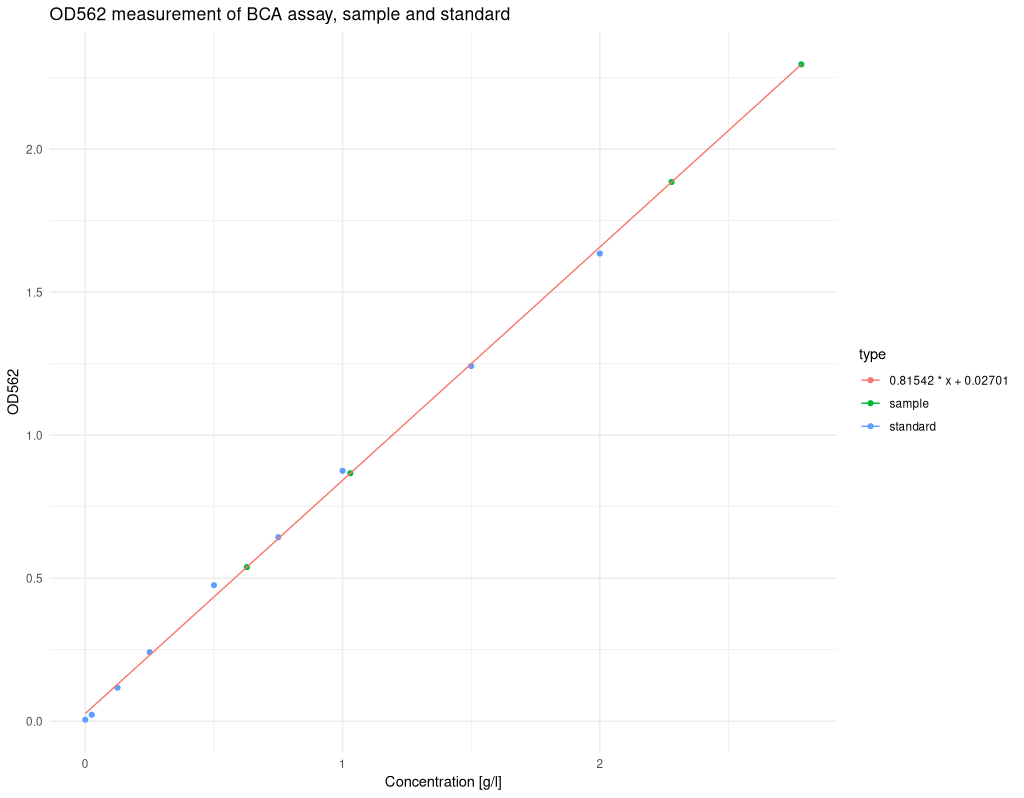
\includegraphics[width=\linewidth]{img/bca_assay.png}
	\caption{OD562 values and concentrations of standard and sample}
	\label{fig:bca_absorption}
\end{figure}

\section{Expression screening}

\subsection{OD measurements during bacterial growth}

To measure the stages of bacterial growth before and after induction, the
absorption at \SI{600}{\nm} was measured in regular intervals. These results are
found in table \ref{tbl:absorption_expression}.

As mentioned in the protocol the measurement at \SI{90}{\min} was faulty, and
was thus excluded from the visualization in figure
\ref{fig:absorption_expression}.

\begin{table}
	\centering
	\begin{tabu}{lllllllll}
		\toprule
		Medium & Rha & IPTG & \SI{0}{\min} & \SI{60}{\min} & \SI{90}{\min} & \SI{120}{\min} & \SI{200}{\min} & \SI{290}{\min} \\
		\midrule
		\csvreader[]{data/expression_od600.csv}%
		{medium=\medium,rha=\rha,iptg=\iptg,4=\tone,5=\ttwo,6=\tthree,7=\tfour,8=\tfive,9=\tsix}%
		{\\ \medium & \rha & \iptg & \tone & \ttwo& \tthree & \tfour & \tfive & \tsix}%
		\\
		\bottomrule
	\end{tabu}
	\caption{OD600 values of transformed bacteria samples}
	\label{tbl:absorption_expression}
\end{table}

\begin{figure}
	\centering
	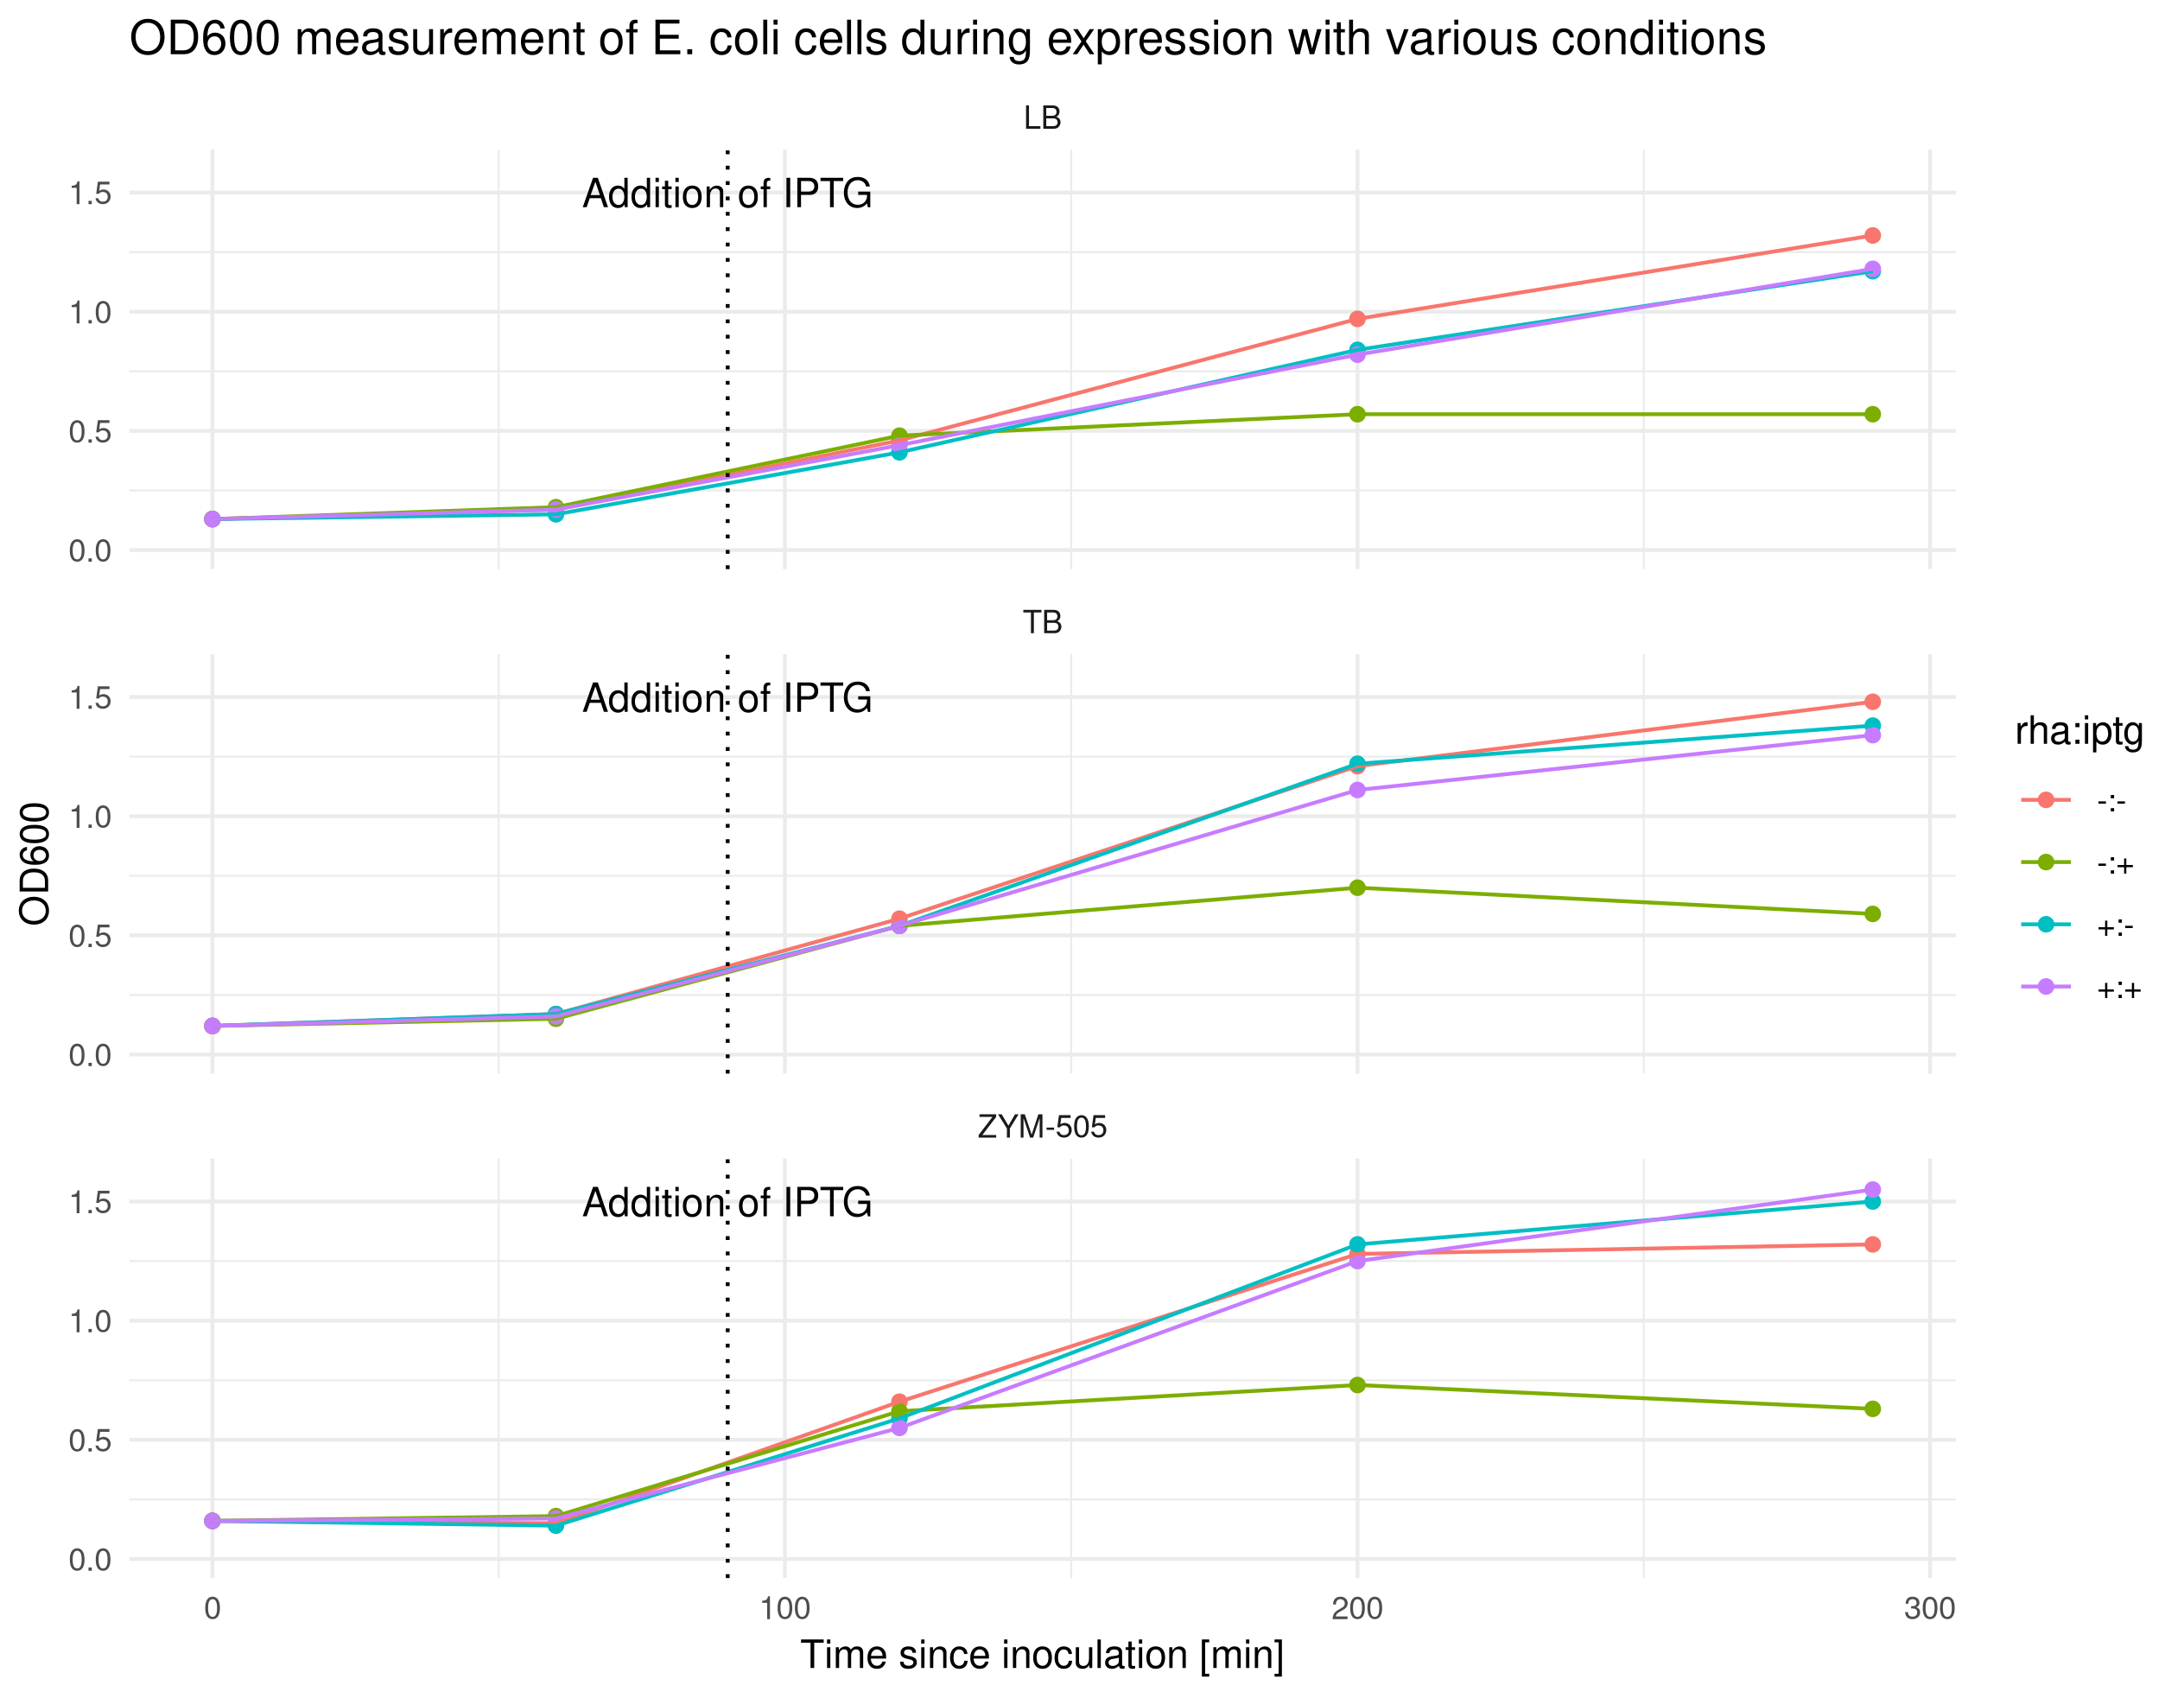
\includegraphics[width=\linewidth]{img/absorption_expression.png}
	\caption{OD600 values over time of expression samples}
	\label{fig:absorption_expression}
\end{figure}

\subsection{Fluorescence measurement}

The fluorescence measurements of the dsRed-marked protein are shown in table
\ref{tbl:expression_fluorescence}. In addition to the measured value this table
also includes the fluorescence normalized to an OD of 1, using the most recent
OD measurements. These values are further visualized in figure
\ref{fig:expression_fluorescence}.

\begin{table}
	\centering
	\begin{tabu}{llllll}
		\toprule
		Medium & Rha & IPTG & Fluorescence & Last OD$_{600}$ & Normalized fluorescence \\
		\midrule
		\csvreader[]{data/expression_fluorescence.csv}%
		{Medium=\medium,Rhamnose=\rha,IPTG=\iptg,Fluorescence=\fluorescence,5=\od,6=\fluorescencenorm}%
		{\\ \medium & \rha & \iptg & \fluorescence & \od & \fluorescencenorm}%
		\\
		\bottomrule
	\end{tabu}
	\caption{Fluorescence values of transformed bacteria samples}
	\label{tbl:expression_fluorescence}
\end{table}

\begin{figure}
	\centering
	\includegraphics[width=\linewidth]{img/expression_fluorescence.png}
	\caption{Fluorescence values of transformed bacteria samples}
	\label{fig:expression_fluorescence}
\end{figure}

\chapter{Discussion}

\section{Isolation of membranes}

The relatively big difference of roughly \SI{20}{\percent} between the two
usable protein concentrations calculated in section
\ref{sec:protein_concentration}, coupled with two of the measurements being
unusable due to being outside the supported range, is not ideal for determining
the concentration of isolated membrane proteins. The big difference in
concentration hints at one of the dilutions being mixed or pipetted
incorrectly. As only two values are available there is further no information
on which dilution was affected.

However, the concentration of either dilution as well as the average thereof
implies that the protein concentration is high enough to achieve the
\SI{10}{\mg\per\ml} required for further purification steps.

\section{Transformation of bacterial cells}

As the colonies were able to grow on a plate treated with kanamycin we can
conclude that the transformation was successful, and the plasmid - which also
confers resistance to kanamycin - was taken in and had been retained.

\section{Expression screening}

\subsection{Bacteria growth}

All references to data in this section refer to figure
\ref{fig:absorption_expression} and table \ref{tbl:absorption_expression}
respectively.

\subsubsection{IPTG- samples}

Samples which were not treated with IPTG showed the typical growth pattern of
bacterial cells. They started with a lag phase without growth, a log phase with
linear growth, and finally a stationary phase where growth stagnated.
Observation stopped before the decline phase, where cell density would have
lowered, was entered.

\subsubsection{IPTG+ samples}

The IPTG+/Rha- sample behaved as expected too. Shortly after IPTG was added it
induced the overexpression of HS, which caused cell growth to stop as all
energy was put towards expression of HS.

The IPTG+/Rha+ sample behaved mostly like the IPTG- samples, which was
unexpected. As Rhamnose leads to the expression of T7 lysozyme, which inhibits
the T7 polymerase\cite{memstar}, we expected the Rha+/IPTG+ sample to exhibit
growth somewhere in between the IPTG- and the Rha-/IPTG+ samples, as the
inhibition of the T7 polymerase would have limited the overexpression of HS,
allowing the cell to continue growing to some extent.

Possible explanations are that either too much Rhamnose was added, such that
the inhibition of the T7 polymerase was too strong, or that none or too little
IPTG had been added. The subsequent analysis of the protein expression using
fluorescence in section \ref{sec:fluorescence} seems to promote the later.

\subsubsection{Medium comparison}

Looking at how fast cell growth was in the different media it is evident that
cells on LB grew the slowest, while cells on TB and ZYM-505 grew at roughly the
same speed. No conclusion can be reached as far as the final cell density is
concerned, as cells did not reach their stationary phase yet.

\subsection{Protein expression}
\label{sec:fluorescence}

All references to data in this section refer to figure
\ref{fig:expression_fluorescence} and table \ref{tbl:expression_fluorescence}
respectively.

\subsubsection{Rha-/IPTG+}

Comparing the normalized fluorescence measurements of the various samples it is
evident that Rha-/IPTG+ samples had the highest protein expression across all
media. This matches the expectation as HS will be expressed fully, without
anything inhibiting it.

\subsubsection{Cell growth on TB}

Further, cells on the TB media seem to have expressed significantly more HS
than on either the LB or ZYM-505 medium. As fluorescence of the Rha-/IPTG-
sample is significantly higher compared to the Rha-/IPTG- samples of the other
two media, it seems likely that this is due to a higher cell density rather
than an increased number of proteins per cell.

\subsubsection{Protein expression on ZYM-505}

Lastly the ZYM-505 medium increased, without promoting general cell growth
unlike the TB medium, the fluorescence of the Rha-/IPTG+ sample. This implies
that, while the number of cells stayed comparable to the LB medium, the number
of HS proteins proteins per cell has increased.

\bibliographystyle{plain}
\bibliography{references}

\end{document}



